%! Author = abenjeddou
%! Date = 30/06/2026

\section{Introduction}
This chapter groups the second and third sprints, as together they cover the data processing aspect of the workflow. It starts with the validation and enrichment of incoming messages, the retrieval of customer subscription records and the application of business rules, and continues with the delivery of notifications to the Erable push notification API and the persistence of the processing state back to Valkey.

\section{Sprint Goals}
The combined goal of these two sprints is to build the core data processing chain of the pipeline:
\begin{itemize}
    \item[-] Validate and deserialize incoming messages, then integrate with the Valkey API to retrieve customer subscription records and apply business rules to determine notification eligibility.
    \item[-] Deliver the eligible notifications to the Erable push notification API and persist the resulting processing state back to Valkey.
\end{itemize}

\section{Logical Pipeline Overview}

\begin{center}
    \centering
    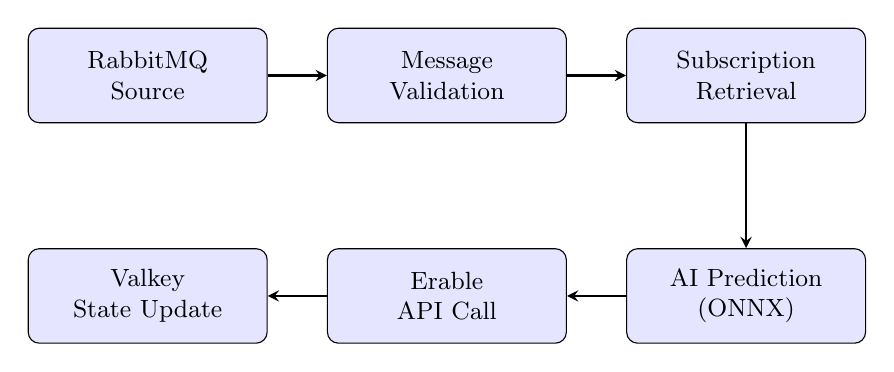
\begin{tikzpicture}[
        node distance=1.8cm,
        block/.style={rectangle, draw, fill=blue!10, text width=2.8cm, text centered, minimum height=1.2cm, rounded corners, font=\small},
        arrow/.style={->, >=stealth, thick}
    ]
        \node[block] (src) {RabbitMQ\\Source};
        \node[block, right of=src, xshift=2cm] (valid) {Message\\Validation};
        \node[block, right of=valid, xshift=2cm] (sub) {Subscription\\Retrieval};
        \node[block, below of=sub, yshift=-1cm] (ai) {AI Prediction\\(ONNX)};
        \node[block, left of=ai, xshift=-2cm] (erable) {Erable\\API Call};
        \node[block, left of=erable, xshift=-2cm] (sink) {Valkey\\State Update};

        \draw[arrow] (src) -- (valid);
        \draw[arrow] (valid) -- (sub);
        \draw[arrow] (sub) -- (ai);
        \draw[arrow] (ai) -- (erable);
        \draw[arrow] (erable) -- (sink);
    \end{tikzpicture}
    \captionof{figure}{LFU job logical pipeline}
    \label{fig:logical-pipeline}
\end{center}

\section{Message Validation and Business Rules}

\subsection{Message Validation and Conversion Operator}

The \texttt{LFUCheckValidMessageFlatMapFunction} class performs three operations:
\begin{enumerate}
    \item \textbf{JSON deserialization}: Converts the raw message into a \texttt{FairUseMessage} object via Jackson.
    \item \textbf{Structural validation}: Verifies Bean Validation constraints (valid French MSISDN, mandatory fields, formats) using Hibernate Validator.
    \item \textbf{Enrichment}: Creates an \texttt{EnrichedFairUseMessage} with a UUID for traceability.
\end{enumerate}

Invalid messages are rejected and counted in the \texttt{discarded\_requests} counter.

\subsection{Subscription Retrieval Operator}

The \texttt{LFUGetSubscriptionProcessFunction} class queries Valkey to retrieve the \texttt{LfuMainRecord} associated with the customer's MSISDN. For each client application (Orange et Moi, My Sosh, Orange Pro), it:
\begin{enumerate}
    \item Verifies that the SID (Service ID) is active via \texttt{isManagedSid()} which checks an environment variable to identify the availability of the service.
    \item Searches for the \textit{main record} in the PushShared table in the subscription database using the \texttt{SubscriptionValkeyDao}.
    \item Validates that the message's event type is compatible with the main record's rules (\texttt{LfuRules}).
\end{enumerate}

\begin{lstlisting}[language=Java, caption={Main record retrieval from Valkey}, breaklines=true]
for (ClientApplication serviceId :
        ClientApplication.values()) {
    String sid = serviceId.getService();
    if (!ClientApplication.isManagedSid(sid)) {
        discardedRequestsCounter.inc();
        continue;
    }
    Optional<LfuMainRecord> lfuMainRecord =
        dao.getLfuMainRecord(msisdn, sid);
    if (lfuMainRecord.isEmpty()) {
        discardedRequestsCounter.inc();
        continue;
    }
    String eventType =
        fairUseMessage.getFairuse().getEventType();
    if (areRulesValid(
            lfuMainRecord.get(), eventType)) {
        notification.setLfuMainRecord(
            lfuMainRecord.get());
        collector.collect(notification);
    }
}
\end{lstlisting}

\subsection{Business Rule Validation}

The \texttt{areRulesValid} method ensures that:
\begin{itemize}
    \item The main record contains a non-null \texttt{LfuRules} object.
    \item The incoming event type (e.g., \texttt{fairuse}, \texttt{blocage}) is present in the subscription's rules' managed events list.
\end{itemize}

Messages failing these checks are discarded with appropriate log codes (\texttt{UNMANAGED\_ EVENT}) and metric increments.

\section{Notification Delivery and State Persistence}

\subsection{Erable API Call Operator}

The \texttt{LFUErableCallProcessFunction} sends the push notification to the Erable system via an HTTP POST call. It:
\begin{enumerate}
    \item Builds the \texttt{LFUErableEntity} containing the MSISDN, customer type, event type, and reached threshold.
    \item Sends the request via Spring \texttt{WebClient} with a configurable retry mechanism.
    \item Only forwards the message downstream if the response is \texttt{2xx}.
    \item Increments per-SID counters (OMOI, SOSH, OPRO) for successful sends.
\end{enumerate}

\begin{lstlisting}[language=Java, caption={HTTP call to Erable}, breaklines=true]
LFUErableEntity body = buildEntity(fairUseMessage);
String erableUri = ErableCallUtils.getPath(
    erableCallConfiguration.getErableHost(),
    erableCallConfiguration
        .getErablePathPattern(), sid);

ResponseEntity<String> response =
    ErableCallUtils.sendErableRequest(
        client, erableUri, erableUuid, body,
        erableCallConfiguration, LOG);

if (response.getStatusCode().is2xxSuccessful()) {
    incrementOmoiOrSoshOrOpro(/* counters */);
    collector.collect(notification);
}
\end{lstlisting}

\subsection{Erable Error Handling}

\begin{itemize}
    \item \textbf{Automatic retry} via \texttt{ErableCallUtils.shouldRetry()} for transient errors (too many requests, connection timeouts, 5xx responses).
    \item \textbf{Critical errors} (e.g., repeated 5xx): exception propagation via \texttt{throwIfCritical Status()} to trigger a Flink restart.
    \item \textbf{Non-critical errors} (e.g., 4xx): log with code \texttt{UNMANAGED\_ERROR} + counter increment, message dropped.
    \item \textbf{Null response}: logged as \texttt{ERABLE\_ACCESS\_ERROR}, message dropped.
\end{itemize}

\subsection{State Update Sink}

The \texttt{LFUUpdateSubscriptionSink} class updates the \texttt{LfuMainRecord}'s state in Valkey with the timestamp of the last processed event. This enables the next processing cycle to compute the time interval since the last notification.

\begin{lstlisting}[language=Java, caption={State update in Valkey}]
lfuMainRecord.getState().setStates(
    Map.of(eventType, Map.of("last", timestamp)));
dao.updateLfuMainRecord(lfuMainRecord);
\end{lstlisting}

\texttt{DataPersistenceException} errors are caught, logged with code \texttt{PERSISTENCE\_LIB\_ ACCESS\_ERROR}, and the per-SID failed counter is incremented.

\section*{Conclusion}

At the end of these two sprints, the core data processing chain was functional end-to-end: messages were consumed from RabbitMQ, validated (rejecting malformed JSON, missing fields, and invalid MSISDN formats), enriched with real subscription data, filtered against business rules, sent to Erable, and their state persisted in Valkey. Messages without a matching main record or with unmanaged event types were correctly discarded. Unit tests with Mockito confirmed correct handling of valid and invalid messages, integration tests validated the Valkey DAO interactions with mocked responses, and the stub mode (\texttt{ERABLE\_STUBBED=true}) allowed testing without a live Erable instance.

